\documentclass[11pt]{article}
\usepackage[margin = 1in]{geometry}
\usepackage{amsmath}
\usepackage{amssymb}
\usepackage{amsthm}
\usepackage{graphicx}
\usepackage{enumitem}
\usepackage{url}
\usepackage[parfill]{parskip}
\usepackage{listings}
\usepackage{caption}
\usepackage{subcaption}
\usepackage[utf8]{inputenc}
\usepackage{xcolor}
\definecolor{codegreen}{rgb}{0,0.6,0}
\definecolor{codegray}{rgb}{0.5,0.5,0.5}
\definecolor{codepurple}{rgb}{0.58,0,0.82}
\definecolor{backcolour}{rgb}{0.95,0.95,0.92}
\lstdefinestyle{mystyle}{
	backgroundcolor=\color{backcolour},   
	commentstyle=\color{codegreen},
	keywordstyle=\color{magenta},
	numberstyle=\tiny\color{codegray},
	stringstyle=\color{codepurple},
	basicstyle=\ttfamily\footnotesize,
	breakatwhitespace=false,         
	breaklines=true,                 
	captionpos=b,                    
	keepspaces=true,                 
	numbers=left,                    
	numbersep=5pt,                  
	showspaces=false,                
	showstringspaces=false,
	showtabs=false,                  
	tabsize=2
}
\lstset{style=mystyle}
\newcommand{\skipline}{\vspace{\baselineskip}}
\newcommand{\spacer}{\noalign{\medskip}}
\newcommand{~}{\sim}
\newcommand{\approches}{\rightarrow}
\newcommand{\qarrow}{\quad \rightarrow \quad}
\newcommand{\qqarrow}{\qquad \rightarrow \qquad}
\newcommand{\qtext}[1]{\quad \text{ #1 } \quad}
\newcommand{\qqtext}[1]{\qquad \text{ #1 } \qquad}
\newcommand{\pard}[2]{\frac{\partial #1}{\partial #2}}
\newcommand{\answer}[1]{\textbf{\boldmath #1}}
\newenvironment{problem}[1]{\textbf{Problem #1: }}{\newpage}

\begin{document}
	
	\begin{center}
		\textbf{Exam 2} \\
		\textbf{Partial Differential Equations} \\
		\textbf{Math 531} \\
		\textbf{Stephen Giang RedID: 823184070} \\
	\end{center}
	I, (\textbf{Stephen Giang}), pledge that this exam is completely my
	own work, and that I did not take, borrow or steal work from any other person, and that I did
	not allow any other person to use, have, borrow or steal portions of my work. I understand that
	if I violate this honesty pledge, I am subject to disciplinary action pursuant to the appropriate
	sections of the San Diego State University Policies.

	\skipline \skipline
	\begin{problem}{1}
		The Laplace equation
		\[\nabla^2u(x,y,z) = 0,\]
		represents the steady-state heat equation without sources. Using circular cylindrical coordinates,
		\[x = r\cos\theta \qquad y=r\sin\theta \qquad z = z\]
		show that the Laplace’s equation is
		\[\frac{1}{r}\pard{}{r}\left(r\pard{u}{r}\right) + \frac{1}{r^2}\pard{^2u}{\theta^2} + \pard{^2u}{z^2} = 0\]
		\newpage
		Notice the following for $r$:
		\[x = r\cos\theta \qarrow \pard{x}{r} = \cos\theta \qquad y = r\sin\theta \qarrow \pard{y}{r} = \sin\theta\]
		\begin{align*}
			\pard{u}{r} &= \pard{u}{x}\pard{x}{r} + \pard{u}{y}\pard{y}{r} = \pard{u}{x}\cos\theta + \pard{u}{y}\sin\theta \\
			\pard{^2u}{r^2} &= \pard{}{r}\left(\pard{u}{x}\right) \cos\theta + \pard{}{r}\left( \pard{u}{y}\right) \sin\theta \\
			&= \left( \pard{}{x}\pard{u}{x}\pard{x}{r} + \pard{}{y}\pard{u}{x}\pard{y}{r}\right)\cos\theta + \left( \pard{}{x}\pard{u}{y}\pard{x}{r} + \pard{}{y}\pard{u}{y}\pard{y}{r}\right) \sin\theta \\
			&= \left(\pard{^2u}{x^2}\cos\theta + \pard{^2u}{y\partial x}\sin\theta\right)\cos\theta + \left( \pard{^2u}{x\partial y}\cos\theta + \pard{^2u}{y^2}\sin\theta\right) \sin\theta \\
			&= \pard{^2u}{x^2}\cos^2\theta + 2\pard{^2u}{y\partial x}\sin\theta\cos\theta + \pard{^2u}{y^2}\sin^2\theta  \\
		\end{align*}
		Notice the following for $\theta$:
		\[x = r\cos\theta \qarrow \pard{x}{\theta} = -r\sin\theta \qquad y = r\sin\theta \qarrow \pard{y}{\theta} = r\cos\theta\]
		\begin{align*}
			\pard{u}{\theta} &= \pard{u}{x}\pard{x}{\theta} + \pard{u}{y}\pard{y}{\theta} = \pard{u}{x}(-r\sin\theta) + \pard{u}{y}(r\cos\theta) \\
			\pard{^2u}{\theta^2} &= \left( \pard{u}{x}(-r\cos\theta) + \pard{u}{y}(-r\sin\theta)\right)  + \left( \pard{}{\theta}\pard{u}{x}(-r\sin\theta) + \pard{}{\theta}\pard{u}{y}(r\cos\theta)\right)  \\
			&= \left( \pard{u}{x}(-r\cos\theta) + \pard{u}{y}(-r\sin\theta)\right) \\
			&\qquad \qquad + \left( \left( \pard{}{x}\pard{u}{x}\pard{x}{\theta} + \pard{}{y}\pard{u}{x}\pard{y}{\theta}\right)(-r\sin\theta) + \left( \pard{}{x}\pard{u}{y}\pard{x}{\theta} + \pard{}{y}\pard{u}{y}\pard{y}{\theta}\right)(r\cos\theta)\right)  \\
			&= \left( \pard{u}{x}(-r\cos\theta) + \pard{u}{y}(-r\sin\theta)\right) \\
			&\qquad \qquad + \left( \left( \pard{^2u}{x^2}(-r\sin\theta) + \pard{^2u}{y\partial x}(r\cos\theta)\right)(-r\sin\theta) + \left( \pard{^2u}{x\partial y}(-r\sin\theta) + \pard{^2u}{y^2}(r\cos\theta)\right)(r\cos\theta)\right)  \\
			&= \left( \pard{u}{x}(-r\cos\theta) + \pard{u}{y}(-r\sin\theta)\right) + \left( \pard{^2u}{x^2}(r\sin\theta)^2 + 2\pard{^2u}{y\partial x}(-r^2\cos\theta\sin\theta) + \pard{^2u}{y^2}(r\cos\theta)^2\right)  \\
			&= -r\left( \pard{u}{x}\cos\theta + \pard{u}{y}\sin\theta\right) + r^2\left( \pard{^2u}{x^2}\sin^2\theta - 2\pard{^2u}{y\partial x}\cos\theta\sin\theta + \pard{^2u}{y^2}\cos^2\theta\right)
		\end{align*}
		\newpage
		Putting it all together, we get:
		\begin{align*}
			\frac{1}{r^2}\pard{^2u}{\theta^2} &= \frac{-1}{r}\pard{u}{r} + \left( \pard{^2u}{x^2}\sin^2\theta - 2\pard{^2u}{y\partial x}\cos\theta\sin\theta + \pard{^2u}{y^2}\cos^2\theta\right) \\
			\pard{^2u}{r^2} + \frac{1}{r^2}\pard{^2u}{\theta^2} &= \frac{-1}{r}\pard{u}{r} + \left( \pard{^2u}{x^2}\sin^2\theta - 2\pard{^2u}{y\partial x}\cos\theta\sin\theta + \pard{^2u}{y^2}\cos^2\theta\right) \\
			&\qquad \qquad \quad + \left(\pard{^2u}{x^2}\cos^2\theta + 2\pard{^2u}{y\partial x}\sin\theta\cos\theta + \pard{^2u}{y^2}\sin^2\theta\right)  \\
			\pard{^2u}{r^2} + \frac{1}{r^2}\pard{^2u}{\theta^2} &= \frac{-1}{r}\pard{u}{r} + \pard{^2u}{x^2} + \pard{^2u}{y^2} \\
			\pard{^2u}{x^2} + \pard{^2u}{y^2} + \pard{^2u}{z^2} &= \pard{^2u}{r^2} + \frac{1}{r}\pard{u}{r} + \frac{1}{r^2}\pard{^2u}{\theta^2} + \pard{^2u}{z^2} \\
			\nabla^2u(x,y,z) &= \frac{1}{r}\pard{}{r}\left(r\pard{u}{r}\right) + \frac{1}{r^2}\pard{^2u}{\theta^2} + \pard{^2u}{z^2} = 0
		\end{align*}
	\end{problem}

	\begin{problem}{2}
		Given the heat equation on a radially symmetric disk
		\[\pard{u}{t} = \frac{k}{r}\pard{}{r}\left(r\pard{u}{r}\right), \qquad 0 < r < a, t > 0,\]
		with boundary condition
		\[u(a,t) = 0, \qquad t > 0,\]
		and initial condition
		\[u(r,0) = f(r), \qquad t > 0\]
		State clearly the implicit boundary conditions. State clearly your Sturm-Liouville problem(s)
		and any orthogonality relationships. Solve this problem (showing the full Fourier series solution
		before applying the initial condition), then using orthogonality relative to the initial condition,
		reduce the Fourier series solution. (Don’t try to reduce your integrals in r.)\\
		\newpage
		Let the following be true:
		\[u(r,t) = \phi(r)h(t) \qquad \phi(a) = 0\]
		Notice the following from separation of variables:
		\[h' + \lambda kh = 0 \qquad \frac{d\phi}{dr} + r\frac{d^2\phi}{dr^2} + \lambda r \phi = 0\]
		Solving the time dependent ODE gives us the following:
		\[h(t) = Ce^{-\lambda k t}\]
		Using a simple scaling transformation of $z = \sqrt{\lambda}r$, we get the following equation fo the spacial ODE:
		\[z^2\frac{d^2\phi}{dr^2} + z\frac{d\phi}{dr} + (z^2 - 0^2)\phi = 0\]
		We can now see that this is a Bessel Differential Equation of order 0:
		\[\phi(r) = c_1J_0(\sqrt{\lambda}r) + c_2Y_0(\sqrt{\lambda}r)\]
		By the boundedness condition, we get that $|\phi(0)| < \infty$, and that $\lim\limits_{z\approches0}Y_0(z) = \pm \infty$, such that $c_2 = 0$:
		\[\phi(r) = c_1J_0(\sqrt{\lambda}r)\]
		Using the boundary condition, we get:
		\[f(a) = 0 = c_1J_0\left(\sqrt{\lambda}a\right)\qqarrow \lambda_{0n}  = \left(\frac{z_{0n}}{a}\right)^2\]
		where $z_{0n}$ is the $n^{th}$ zero of $J_0$.
		\\ \\
		Now we get the following for $u$:
		\[u(r,t) = \sum_{n = 1}^{\infty} A_nJ_0\left(\sqrt{\lambda_{0n}}r\right)e^{-\lambda_{0n} k t}\]
		Now if we use the initial condition, we get the following:
		\[u(r,0) = f(r) = \sum_{n = 1}^{\infty} A_nJ_0\left(\sqrt{\lambda_{0n}}r\right)\]
		Now we can solve for the following coefficient:
		\[A_n = \frac{\int_{0}^{a}f(r)J_0\left(\sqrt{\lambda_{0n}}r\right)r\,dr}{\int_{0}^a J_0^2\left(\sqrt{\lambda_{0n}}r\right)r\,dr}\]
	\end{problem}

	\begin{problem}{3}
		\begin{enumerate}[label = (\alph*)]
			\item Solve the heat equation on a disk
			\[\pard{u}{t} = \frac{1}{r}\pard{}{r}\left(r\pard{u}{r}\right) + \frac{1}{r^2}\pard{^2u}{\theta^2}, \qquad 0 < r < 1, \quad -\pi < \theta < \pi, \quad t > 0, \]
			with the boundary condition
			\[u(1,\theta,t) = \sin 3\theta,\]
			and the initial condition
			\[u(r,\theta,0) = 0\]
			State clearly the implicit boundary conditions. State clearly your Sturm-Liouville problem(s)
			and any orthogonality relationships. Solve this problem (showing the full Fourier series solution
			before applying the initial condition), then using orthogonality relative to the initial condition,
			reduce the Fourier series solution. (Don’t try to reduce your integrals in r.)
			\newpage
			Let the following be true:
			\[u(r,\theta,t) = f(r)g(\theta)h(t)\]
			Using separation of variables, we get the following three equations:
			\[h' = -\lambda h \qquad g'' = -\mu g \qquad r\frac{d}{dr}\left(r \frac{df}{dr}\right) + (\lambda r^2 - \mu)f = 0\]
			Solving the time dependent ODE, we get:
			\[h(t) = Ce^{-\lambda t}\]
			Solving the angular ODE, we get the following eigenvalue and eigenfunctions:
			\[\mu = m^2 \qquad g(\theta) = a_m\cos m\theta + b_m\sin m\theta\]
			Using a simple scaling transformation of $z = \sqrt{\lambda}r$, we get the following equation fo the radial ODE:
			\[z^2\frac{d^2f}{dr^2} + z\frac{df}{dr} + (z^2 - m^2)f = 0\]
			We can now see that this is a Bessel Differential Equation of order $m$:
			\[f(r) = c_1J_m(\sqrt{\lambda}r) + c_2Y_m(\sqrt{\lambda}r)\]
			By the boundedness condition, we get that $|f(0)| < \infty$, and that $\lim\limits_{z\approches0}Y_0(z) = \pm \infty$, such that $c_2 = 0$:
			\[f(r) = c_1J_m(\sqrt{\lambda}r)\]
			Now we get the following for $u$:
			\[u(r,\theta,t) = \sum_{m = 0}^{\infty} \sum_{n = 1}^{\infty} A_{mn}J_m\left(\sqrt{\lambda}r\right)\cos m\theta\,e^{-\lambda t} + \sum_{m = 0}^{\infty} \sum_{n = 1}^{\infty} B_{mn}J_m\left(\sqrt{\lambda}r\right)\sin m\theta\,e^{-\lambda t}\]
			Now if we use the boundary condition, we get the following:
			\[u(1,\theta, t) = \sin 3\theta = \sum_{m = 0}^{\infty} \sum_{n = 1}^{\infty} A_{mn}J_m\left(\sqrt{\lambda}\right)\cos m\theta\,e^{-\lambda t} + \sum_{m = 0}^{\infty} \sum_{n = 1}^{\infty} B_{mn}J_m\left(\sqrt{\lambda}\right)\sin m\theta\,e^{-\lambda t}\]
			We can now see that $m = 3$:
			\[1 = \sum_{n = 1}^{\infty} A_{3n}J_3\left(\sqrt{\lambda_{3n}}\right)\,e^{-\lambda_{3n} t}\]
			Now we can solve for the following coefficient:
			\[A_{3n} = \frac{\int_{0}^{a}J_3\left(\sqrt{\lambda_{3n}}r\right)r\,dr}{e^{-\lambda_{3n} t} \int_{0}^a J_3^2\left(\sqrt{\lambda_{3n}}r\right)r\,dr}\]
			\\ \\
			\newpage
			\item Find the steady-state temperature in the disk.
			\\ \\
			The disk has a radius of 1. The upper half of the circumference is kept at
			$100^\circ$ and the lower half is kept at $0^\circ$
			\begin{figure}[h!]
				\centering
				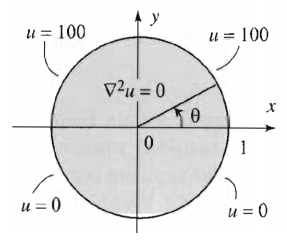
\includegraphics[width=.4\linewidth, height=.25\textheight]{Prob3b.png}
			\end{figure}
		\end{enumerate}
	\end{problem}

	\begin{problem}{4}
		 Consider heat conduction in a sphere given by:
		\[\pard{u}{t} = k\left(\frac{1}{\rho^2}\pard{}{\rho}\left(\rho^2 \pard{u}{\rho}\right) + \frac{1}{\rho^2\sin\phi}\pard{}{\phi}\left(\sin\phi\pard{u}{\phi}\right) + \frac{1}{\rho^2\sin\phi}\pard{^2u}{\theta^2}  \right),\]
		\[0 < \rho < a, \quad -\pi < \theta \leq \pi, \quad 0 \leq \phi \leq \pi,\quad t > 0\]
		with the boundary condition
		\[\pard{u}{\rho}(a,\theta,\phi,t) = 0,\]
		and initial conditions:
		\[u(\rho,\theta,\phi,0) = F(\rho,\phi)\sin3\theta\]
		Solve this equation noting any other boundary conditions you might need to apply. State clearly
		your Sturm-Liouville problem(s) and any orthogonality relationships.
		\newpage
		Notice the following separation of variables:
		\[u(\rho,\theta,\phi,t) = w(\rho,\theta,\phi)h(t) = f(\rho)q(\theta)g(\phi)h(t)\]
		From this, and our original equation, we get the following time equation:
		\[h' + \lambda k t = 0\]
		Notice the following spatial equations:
		\[q'' + \gamma q = 0 \qquad \frac{d}{d\rho}\left(\rho^2 \frac{df}{d\rho}\right) + \left(\lambda \rho^2 - \mu\right)f = 0 \qquad \frac{d}{d\phi}\left(\sin\phi \frac{dg}{d\theta}\right) + \left(\mu \sin\phi - \frac{m^2}{\sin\phi}\right)g = 0\]
		Notice the solution to the time dependent ODE:
		\[h(t) = Ce^{-\lambda k t}\]
		Notice from the $\theta$ dependent ODE, we get the following eigenvalues and eigenfunctions:
		\[\gamma = m^2 \qquad q(\theta) = a_m\cos m\theta + b_m \sin m\theta\]
		Notice the radial ODE, if we let $\mu = n(n + 1)$:
		\[\frac{d}{d\rho}\left(\rho^2 \frac{df}{d\rho}\right) + \left(\lambda \rho^2 - n(n+1)\right)f = 0 \qqarrow f(\rho) = \rho^{-1/2}J_{n + \frac{1}{2}}\left(\sqrt{\lambda}\rho\right) \]
		Using the boundary condition $f(a) = 0$, we get:
		\[\lambda_{mn} = \left( \frac{z_{mn}}{a}\right) ^2\]
		Notice the $\phi$ dependent ODE, if we let $x = \cos \theta$, we get the following:
		\[\frac{d}{dx}\left((1-x^2)\frac{dg}{dx}\right) + \left( n(n+1) - \frac{m^2}{1-x^2}\right)g = 0 \qarrow g(x) = P_n^m\left( \cos \theta\right) \]
		\newpage
		Thus, we get the following for $u$:
		\begin{align*}
			u(\rho,\theta,\phi,t) &= \sum_{m = 0}^\infty \sum_{n = 1}^\infty A_{mn}\rho^{-1/2}J_{n + \frac{1}{2}}\left(\sqrt{\lambda_{mn}}\rho\right)P_n^m\left( \cos \theta\right)\cos m\theta\,e^{-\lambda k t} \\
			&+ \sum_{m = 0}^\infty \sum_{n = 1}^\infty B_{mn}\rho^{-1/2}J_{n + \frac{1}{2}}\left(\sqrt{\lambda_{mn}}\rho\right)P_n^m\left( \cos \theta\right)\sin m\theta\,e^{-\lambda k t}
		\end{align*}
		Using our initial condition, we get:
		\begin{align*}
			u(\rho,\theta,\phi,0) = F(\rho,\phi)\sin 3\theta &= \sum_{m = 0}^\infty \sum_{n = 1}^\infty A_{mn}\rho^{-1/2}J_{n + \frac{1}{2}}\left(\sqrt{\lambda_{mn}}\rho\right)P_n^m\left( \cos \theta\right)\cos m\theta \\
			&+ \sum_{m = 0}^\infty \sum_{n = 1}^\infty B_{mn}\rho^{-1/2}J_{n + \frac{1}{2}}\left(\sqrt{\lambda_{mn}}\rho\right)P_n^m\left( \cos \theta\right)\sin m\theta \\
			&= \sum_{n = 1}^\infty B_{3n}\rho^{-1/2}J_{n + \frac{1}{2}}\left(\sqrt{\lambda_{3n}}\rho\right)P_n^3\left( \cos \theta\right)\sin 3\theta 
		\end{align*}
		Thus, we get the following:
		\[F(\rho,\phi) = \sum_{n = 1}^\infty B_{3n}\rho^{-1/2}J_{n + \frac{1}{2}}\left(\sqrt{\lambda_{3n}}\rho\right)P_n^3\left( \cos \theta\right)\]
		and the following coefficients:
		\[B_{3n} = \frac{\int_{0}^{a}F(\rho,\phi)J_{n + \frac{1}{2}}\left(\sqrt{\lambda_{3n}}r\right)r\,dr}{\rho^{-1/2}P_n^3(\cos \theta)\int_{0}^a J_{n + \frac{1}{2}}^2\left(\sqrt{\lambda_{3n}}r\right)r\,dr}\]
	\end{problem}

	\begin{problem}{5}
		Find the steady-state temperature in a cube, which satisfies:
		\[\nabla^2u(x,y,z) = 0, \qquad 0 < x < a, \quad 0 < y < b, \quad 0 < z < c.\]
		The cube is kept at $0^\circ$C on all faces except on the upper horizontal face. 
		\begin{figure}[h!]
			\centering
			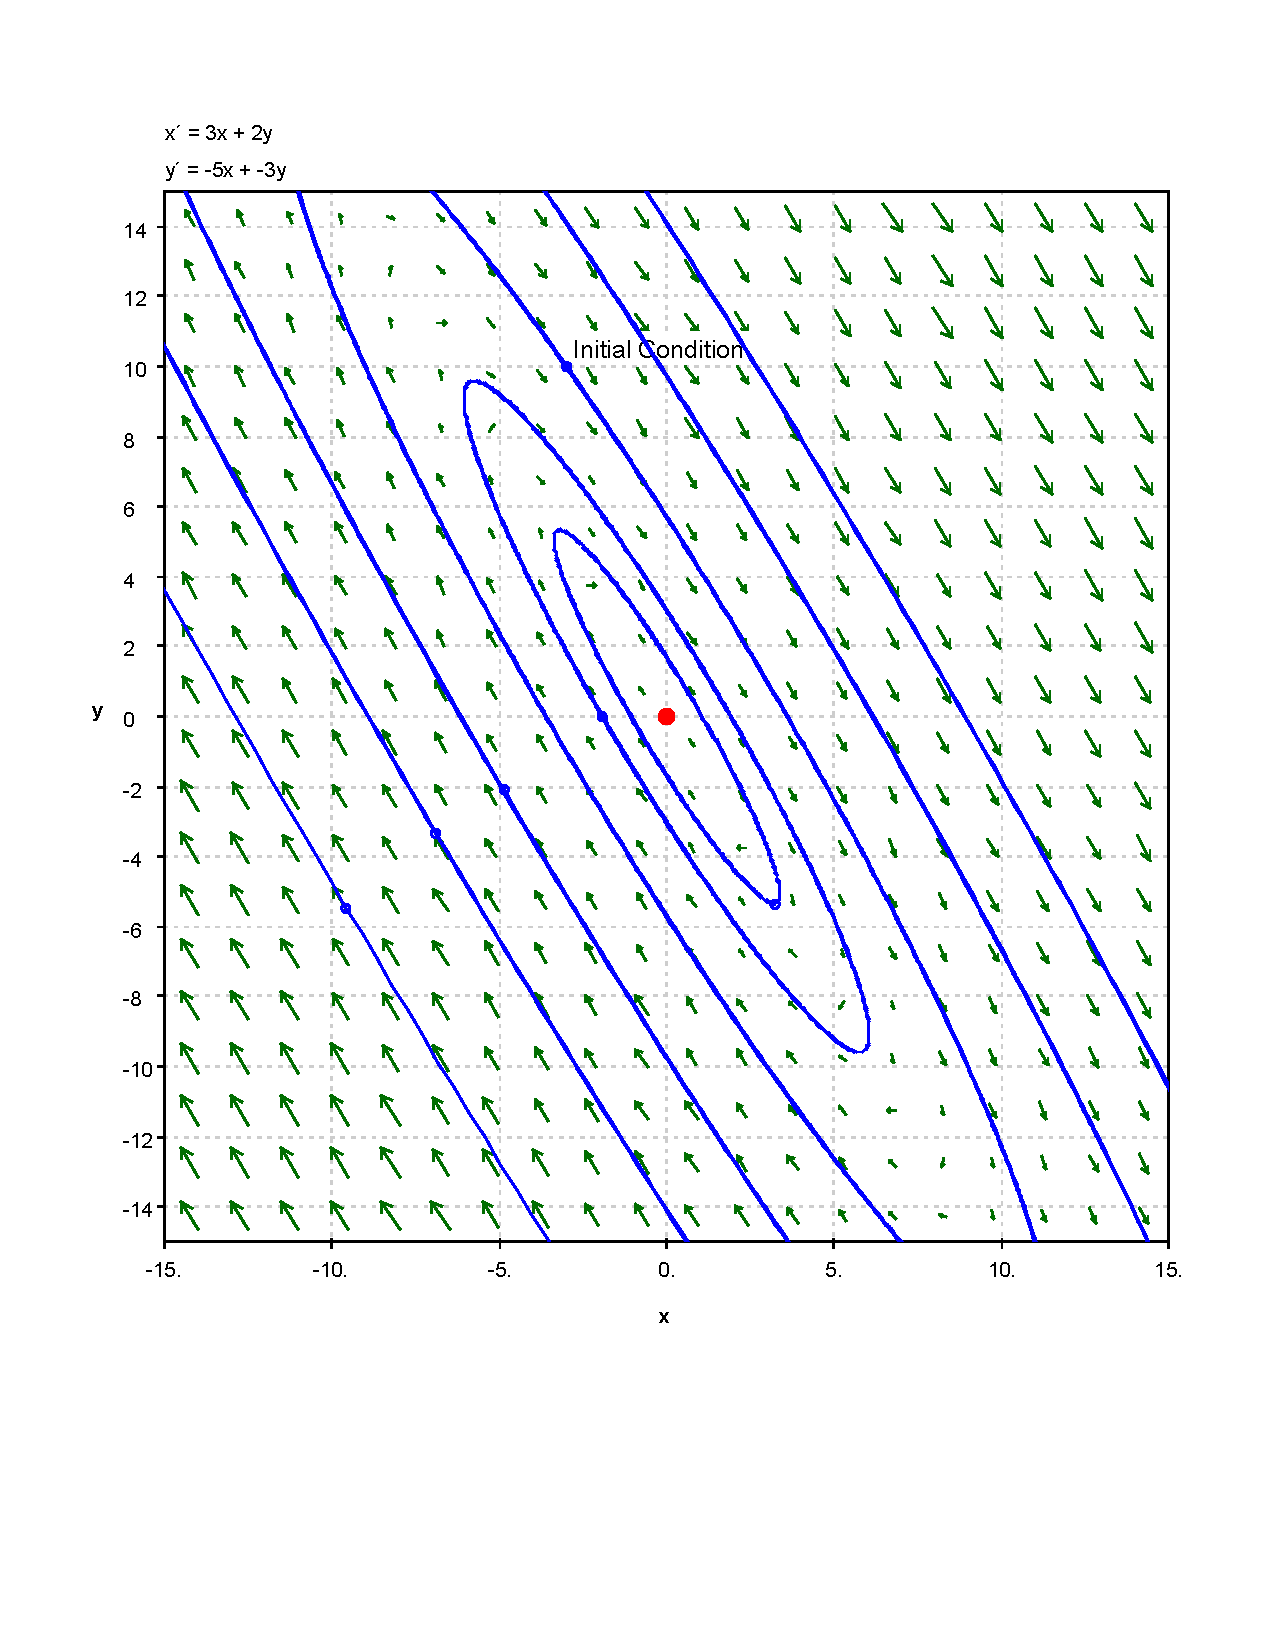
\includegraphics[width=.4\linewidth, height=.25\textheight]{Prob5.png}
		\end{figure}
		\newpage
		Notice the following:
		\[\nabla^2u(x,y,z) = \pard{^2u}{x^2} + \pard{^2u}{y^2} + \pard{^2u}{z^2} = 0\]
		Now we let the following be true:
		\[u(x,y,z) = f_1(x)g(y)h(z)\]
		And we get the following from separation of variables:
		\[f_1'' = -\lambda f_1 \qquad g'' = -\mu g \qquad h'' - (\lambda  + \mu)h = 0\]
		Notice the following for the $x$ dependent equation, we get:
		\[f_1(x) = a_1\cos\sqrt{\lambda}x + a_2\sin\sqrt{\lambda}x\]
		Now we apply the following boundary conditions, $f_1(0) = f_1(a) = 0$:
		\[f_1(0) = a_1 = 0 \qquad f_1(a) = a_2\sin\sqrt{\lambda}a \qquad \lambda_n = \left( \frac{n\pi}{a}\right) ^2\]
		Notice the following for the $y$ dependent equation, we get:
		\[g(y) = b_1\cos\sqrt{\mu}y + b_2\sin\sqrt{\mu}y\]
		Now we apply the following boundary conditions, $g(0) = g(b) = 0$:
		\[g(0) = b_1 = 0 \qquad f(b) = b_2\sin\sqrt{\mu}b \qquad \mu_m = \left( \frac{m\pi}{b}\right) ^2\]
		Notice the following for the $z$ dependent equation, we get:
		\[h(z) = c_1\cosh(\sqrt{\lambda + \mu}z) + c_2\sinh(\sqrt{\lambda + \mu}z)\]
		Now we use our boundary condition, $h(0) = 0$, to get $c_1 = 0$:
		\[h(z) = c_2\sinh(\sqrt{\lambda + \mu}z)\]
		\newpage
		Thus we get the following for $u$:
		\[u(x,y,z) = \sum_{m = 1}^\infty \sum_{n = 1}^\infty A_{mn}\sin\frac{n\pi x}{a}\sin\frac{m\pi x}{b}\sinh(\sqrt{\lambda_{n} + \mu_m}z)\]
		Using our other boundary condition, we get:
		\[u(x,y,c) = f(x,y) = \sum_{m = 1}^\infty \sum_{n = 1}^\infty A_{mn}\sin\frac{n\pi x}{a}\sin\frac{m\pi x}{b}\sinh(\sqrt{\lambda_{n} + \mu_m}c)\]
		From here, we can solve for the following coefficient:
		\[A_{mn} = \frac{4}{ab\sinh(\sqrt{\lambda_{n} + \mu_m}c)}\int_{0}^{a} \int_{0}^b \sin\frac{n\pi x}{a}\sin\frac{m\pi x}{b} f(x,y)\,dy\,dx\]
	\end{problem}

	\begin{problem}{6}
		 Solve the heat equation
		 \[\pard{u}{t} = k\left(\frac{1}{r}\pard{}{r}\left(r\pard{u}{r}\right) + \pard{^2u}{z^2} \right), \qquad 0 < r < 2, \quad 0 < z < 7, \quad t > 0, \]
		 inside a cylinder subject to the initial condition
		 \[u(r,z,0) = 100,\]
		 if the boundary conditions are:
		 \[u(2,z,t) = 0, \quad u(r,0,t) = 0, \quad u(r,7,t) = 100\]
		 \newpage
		 We can separate the original equation and get the following:
		 \[u(r,z,t) = f(r)g(z)h(t)\]
		 From here, we get the following, from separating the variables:
		 \[h' = -\lambda k t \qquad g'' = -\gamma g \qquad r\left(\frac{d}{dr}\left(r \frac{df}{dr}\right) \right) + \left( \lambda - \gamma\right) r^2f\]
		 Solving the time equation, gives us the following:
		 \[h(t) = Ce^{-\lambda kt}\]
		 Solving the height equation gives us the following eigenvalues and eigenfunctions:
		 \[\gamma = m^2 \qquad g(z) = a_m \cos m z + b_m \sin m z\]
		 Using the homogeneous boundary condition, we get $a_m = 0$, such that:
		 \[g(z) = b_m \sin m z\]
		 Solving the radial equation, and using the boundedness condition, gives us the following:
		 \[f(r) = c_1J(\sqrt{\lambda}r)\]
		 Using the boundary condition, we get:
		 \[\lambda_{mn} = \left(\frac{z_{mn}}{2}\right)^2\]
		 Thus we get the following for $u$:
		 \[u(r,z,t) = \sum_{m = 0}^\infty \sum_{n = 1}^\infty B_{mn}J(\sqrt{\lambda_{mn}}r)e^{-\lambda_{mn} kt}\sin m z\]
		 Now we include our nonhomogeneous boundary equations:
		 \[u(r,7,t) = \sum_{m = 0}^\infty \sum_{n = 1}^\infty B_{mn}J(\sqrt{\lambda_{mn}}r)e^{-\lambda_{mn} kt}\sin 7m = 100\]
		 \[u(r,z,0) = \sum_{m = 0}^\infty \sum_{n = 1}^\infty B_{mn}J(\sqrt{\lambda_{mn}}r)\sin mz = 100\]
	\end{problem}

	\begin{problem}{7}
		 Find the eigenvalues and eigenfunctions which arise from the Sturm-Liouville problem:
		 \[x\frac{d}{dx}\left(x\frac{d\phi}{dx}\right) + \left(\lambda x^2 - 9\right)\phi = 0, \qquad  0 < x < 6,  \]
		 with $\phi'(6) = 0$ and $\phi(x)$ bounded for $x \in [0, 6]$. Clearly state the orthogonality relationship for
		 the eigenfunctions and use the eigenfunctions to find the Fourier expansion for a function $f(x)$.
		 Give an integral expression for the Fourier coefficients. Assume that
		 \[f(x) = \begin{cases}
		 	x, & x < \frac{1}{2}, \\ 1 - x, & x > \frac{1}{2}
		 \end{cases}\]
	 	 \newpage
	 	 We can see that $m = 3$ here, such that we get the following for $\phi$:
	 	 \[\phi(x) = c_1J_3(\sqrt{\lambda}x) + c_2Y_3(\sqrt{\lambda}x)\]
	 	 The boundedness condition tells us that $c_2 = 0$, such that:
	 	 \[\phi(x) = c_1J_3(\sqrt{\lambda}x)\]
	 	 We can also use our boundary condition to get:
	 	 \[\phi'(x) = c_1\sqrt{\lambda}J_3(\sqrt{\lambda}x) \qqarrow \phi'(6) = 0 = c_1\sqrt{\lambda}J_3(6\sqrt{\lambda}) \qqarrow \lambda = \left(\frac{z_{3n}}{6}\right)^2\]
	\end{problem}


\end{document}
